\begin{figure*}[!t]
\centering
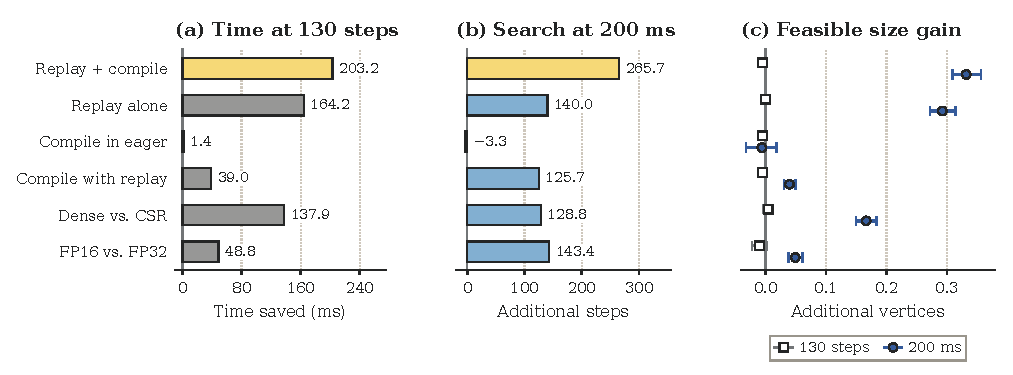
\includegraphics[width=.95\textwidth]{figures/execution_effects.pdf}
\caption{\textbf{How execution changes SPRINT-S.} Each row compares matched runs on 1,000 small RB graphs and three seeds. Gold bars mark the joint switch from eager, uncompiled execution to compiled CUDA Graph replay. The next three rows separate these switches. Both adjacency formats use uncompiled replay. The precision comparison uses compiled replay with TF32 disabled. (a) Time saved at 130 steps. (b) Additional steps within 200~ms. (c) Mean paired gain in delivered size under each protocol, with pointwise 95\% graph-bootstrap intervals.}
\label{fig:execution-effects}
\end{figure*}
